\chapter{Entwicklung}

\section{Backend}

\subsection{Spiellogik}

Die übergeordnete Struktur zum Spielen in der Anwendung ist ein Lobby-System. Dabei werden die Lobbies, also beispielsweise deren Erstellung und Löschung, vom Lobby-Manager verwaltet, das eigentliche Spielen wird über einzelne Lobbies an sich organisiert. Es muss also zuerst eine Lobby erstellt werden, welcher alle Mitspieler entsprechend beitreten können. In dieser können dann Spieleinstellungen wie die gewünschte Edition oder die Rundenanzahl eingestellt werden. Schlussendlich kann in der Lobby ein Spiel begonnen werden, welches im Backend dann ungefähr wie im vereinfachten und groben Sequenzdiagramm in \cref{fig:game-flow} zu sehen ist, abläuft.

\begin{figure}
	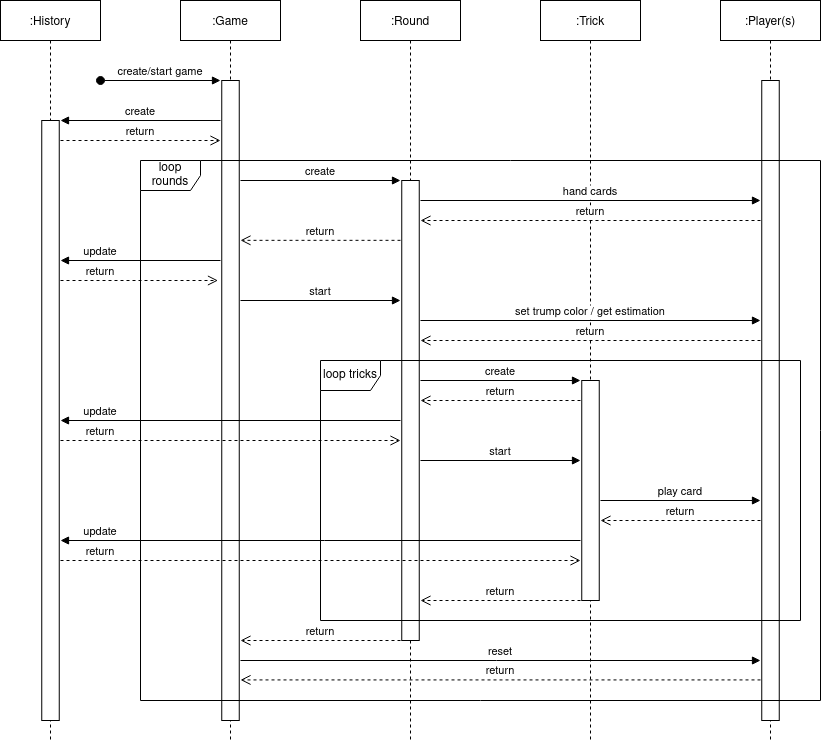
\includegraphics[width=\textwidth]{images/game-flow.png}
	\caption{Spielablauf}
	\label{fig:game-flow}
\end{figure}

Die Spiellogik besteht also elementar aus den Objekten Spiel, Runde, Stich, Spieler und Karte. Dabei wird ein Spiel mit einer Liste an Spielern erstellt und eine Game-Loop gestartet:

\begin{lstlisting}[language=Python]
while self.round_counter <= self.settings.round_number:
	self.curr_round = Round(history=self.history, first_player=self.first_player, round_counter=self.round_counter)
	self.history.update_round(self.curr_round)
	await self.__do_round()
\end{lstlisting}

\begin{lstlisting}[language=Python]
async def __do_round(self):
	await self.curr_round.start_round()
	self.first_player = (self.first_player + 1) % len(self.players)
	self.round_counter += 1
	self.history.save_round()
	for p in self.players.values(): p.reset()
\end{lstlisting}

Wie hier zu sehen ist, erstellt die Game-Loop grundsätzlich pro Runde ein neues Runden-Objekt und "startet" dieses. Nachdem bei Erstellung der Runde bereits Karten verteilt und die Trumpfkarte bestimmt werden, geschieht innerhalb einer Runde Folgendes:

\begin{lstlisting}[language=Python]
async def start_round(self):
	await self.__init_trump()
	await self.__get_estimations()
	
	for i in range(1, self.round_number + 1):
		self.curr_trick = Trick(history=self.history, first_player=self.first_player, trick_number=i, trump_color=self.trump_color)
		self.history.add_trick(self.curr_trick)
		winning_player, after_effects = await self.curr_trick.do_trick()
		await asyncio.sleep(2)
		self.first_player  = winning_player.pos
		await self.__handle_after_effects(after_effects, winning_player, i)
	self.__calculate_points()
\end{lstlisting}

Eine Runde besteht also darin, die Trumpffarbe der Runde zu bestimmen, die Spieler ihre Stich-Schätzung abgeben zu lassen und dann die nötige Anzahl an Stichen durchführen zu lassen. Dafür werden jeweils Stich-Objekte erstellt und "ausgeführt":

\begin{lstlisting}[language=Python]
async def do_trick(self) -> tuple[Player, list[str]]:
	players: list[Player] = self.history.get_players()
	for _ in players:
		await self.__play_card()
		self.history.update_trick(self)
	return (self.get_current_winner(), self.__get_after_effects())
\end{lstlisting}

Hier wird also schlussendlich jeder Spieler nacheinander dazu aufgefordert, eine Karte zu spielen und der Gewinner des Stichs ermittelt.

In den obigen Ausschnitten sind außerdem noch zwei wichtige Aspekte zu erkennen. Zum einen ist an den Schlüsselwörtern "async" und "await" zu erkennen, dass die interaktive und daher asynchrone Natur eines Spiels mittel "asyncio" realisiert wurde. Zum anderen taucht immer wieder eine "history" auf. Dabei handelt es sich um ein Objekt, welches den Spielverlauf enthält und damit zwei aufgekommene Problematiken löst. Der erste Zweck dieser Klasse ist die Lösung des Problems synchroner Datenabfragen in einem asynchronen System. Es wird also sichergestellt, dass mit der Spiellogik konsistente Antworten auf API-Anfragen geliefert werden können. Daher wird, sobald sich die Daten eines relevanten Objekts, beispielsweise eines Stichs, ändern, eine entsprechende Funktion der History zum aktualisieren dieser Daten aufgerufen. So kann die History als zentrale Datenquelle für die API dienen und dabei mit entsprechenden Lock-Mechanismen vor Inkonsistenzen geschützt werden. Die andere Aufgabe dieses Objekts ist die maximale Minderung der nötigen Datenbank-Aufrufe, und die Ereignisse eines Spiels abzuspeichern. Genauer kann, dadurch, dass die History den gesamten Spielverlauf enthält, am Ende eines Spiels ein einziger Datenbank-Aufruf zum Speichern des Spiels erfolgen und alle relevanten Daten werden direkt gespeichert.

Die gesamte Spiellogik kann dabei unter /backend/game und /backend/lobby gefunden werden.

\subsection{API}
Für die API kam das Web-Framework \textit{FastAPI} zum Einsatz. Hierbei wurden folgende Routen definiert:

\subsubsection{GET /\{full\_path:path\}}
Die Aufgabe dieser Route ist es, beim Deployment die Ressourcen an das Frontend liefern zu können. Dabei wird zwischen \textit{privaten} und \textit{öffentlichen} Dateien unterschieden. Erstere benötigen eine valide Authentifizierung, Letztere nicht. Diese Überprüfung verläuft über einen Abgleich der Cookies, wobei der Cookie vom Nutzer über die von der FastAPI bereitgestellten Klasse \textit{Request} abgerufen werden kann. Zudem wird sichergestellt, dass die angefragte Ressource niemals den Ordner \textit{static} verlässt. Falls die geforderten Dateien nicht existieren, wird standardmäßig \textit{index.html} versendet, damit auch die Routen im Frontend wie gewünscht funktionieren. Um die Datei letztendlich zu verschicken, wird die von FastAPI mitgelieferte Klasse \textit{FileResponse} genutzt, welche einen asynchronen Datentransfer ermöglicht. \cite{fastapi-fileresponse}

\subsubsection{POST /api/gql}
Um einen Austausch von Daten beziehungsweise Status zwischen Frontend und Backend zu ermöglichen, fiel die Wahl auf die Abfragesprache \textit{GraphQL}. Für die einfachere Programmierung wurde ein Python-Dekorateur namens \textit{smart\_api} entwickelt, welcher je nach Wunsch repetitive Aufgaben wie beispielsweise 
\begin{itemize}
	\item Authentifizierung, 
	\item Caching
	\item Auflösung von Abhängigkeiten wie zum Beispiel die Datenbank, den Lobby-Manager oder auch das für den Spieler aktive Spiel
\end{itemize}
erledigt. Dabei stellt die API folgende Leseabfragen zur Verfügung:

\begin{lstlisting}
type Query {
	# user management
	loginInformation(name: String!): LoginInformation
	user(id: ID!): User
	whoami: User
	
	# lobby management
	lobby: Lobby
	modes: [String!]!
	
	# game logic
	gameInfo: GameInfo
	gameOver: Boolean
	requiredAction: RequiredAction
	
	# misc
	appointments: [Appointment!]!
	
	# statistics
	residentSleeper: ResidentSleeper!
}
\end{lstlisting}

Zusätzlich dazu sind Schreibabfragen wie folgt möglich:

\begin{lstlisting}
type Mutation {
	# user management
	register(name: String!, passwordHash: String!, salt: String!, 
		hashType: String!, token: String!): Boolean!
	login(name: String!, passwordHash: String!, 
		stayLoggedIn: Boolean! = false): User
	logout: Boolean!
	
	# lobby management
	createLobby: String!
	setLobbySettings(mode: String, roundLimit: Int): Boolean!
	joinLobby(code: String!): Boolean!
	leaveLobby: Boolean!
	startGame: Boolean!
	endGame: Boolean!
	
	# game logic
	completeAction(option: String!): Boolean!
	
	# misc
	joinAppointment(id: ID!) Boolean!
	leaveAppointment(id: ID!) Boolean!
	createAppointment(start: String!, end: String!) Boolean!
}
\end{lstlisting}

\subsection{Datenbank}
Um Informationen über die Spiele, Termine, Spieler und Login-Informationen zu speichern, kam die in der Python-Standardbibliothek enthaltene Offline-Datenbank SQLite zum Einsatz. Für die Anbindung im Backend fiel die Entscheidung auf eine \textit{asyncio}-Implementation, da gewisse Abfragen auf die Datenbank Lese- beziehungsweise Schreiboperation auslösen können, welche immer eine gewisses Maß an Wartezeit im Code zur Folge haben. Die Python Klasse \textit{Database}, welche die fortgeschrittenere Anbindung zur eigentlichen Datenbank bietet, initialisiert zu Beginn einen \textit{Thread-Pool} mit einem Thread, welcher ausschließlich für die Datenbankoperationen reserviert ist. Durch diesen Ansatz müssen die einzelnen Abfragen nicht synchronisiert werden und können direkt mit dem \textit{asyncio} Paket integriert werden.

\begin{lstlisting}[language=Python]
db = Database("wizard.db") # Der Dateiname
await db.login(name="user", password_hash="...")
\end{lstlisting}

Durch diesen Ansatz kann Pythons Coroutinen-Implementierung einen einzelnen Thread besser auslasten, da Operationen, welche mit Warten verbunden sind, in den Hintergrund geschoben werden.

Für die Benutzerregistrierung existieren zwei Methoden namens \textit{register\_user} und \textit{consume\_token}. Die erste Methode legt einen neuen Benutzer in der Datenbank an und speichert hierbei den Namen, einen Hash vom Passwort, sowie den dazugehörigen Salt (siehe \cref{fig:user-db}). \textit{consume\_token} ermöglicht es dem Backend eine Registrierung nur mit gültigem Token zu erlauben. Hierbei wird der vom Benutzer eingegebene Registriertoken mit den Token in der Datenbank abgeglichen und je nach Resultat wird der Token gelöscht und die Registrierung erlaubt oder abgewiesen. Dies soll unerwünschte Anmeldungen verhindern.

Die eigentliche An- und Abmeldung der Benutzer ist etwas komplexer, was sich auch in der Anzahl der benötigten Methoden widerspiegelt: \textit{login}, \textit{logout}, \textit{is\_logged\_in}, \textit{get\_user\_by\_cookie} und \textit{get\_login\_information}. Bevor sich ein Nutzer anmelden kann muss dieser durch \textit{get\_login\_information} essentielle Informationen abfragen, wie einen Salt-Wert der für die Schlüsselgenerierung wichtig ist. In keinem Fall wird das eigentliche Benutzerpasswort an das Backend gesendet oder anderweitig gespeichert (siehe \cref{sec:frontend-registrierung}).

\begin{figure}[h]
	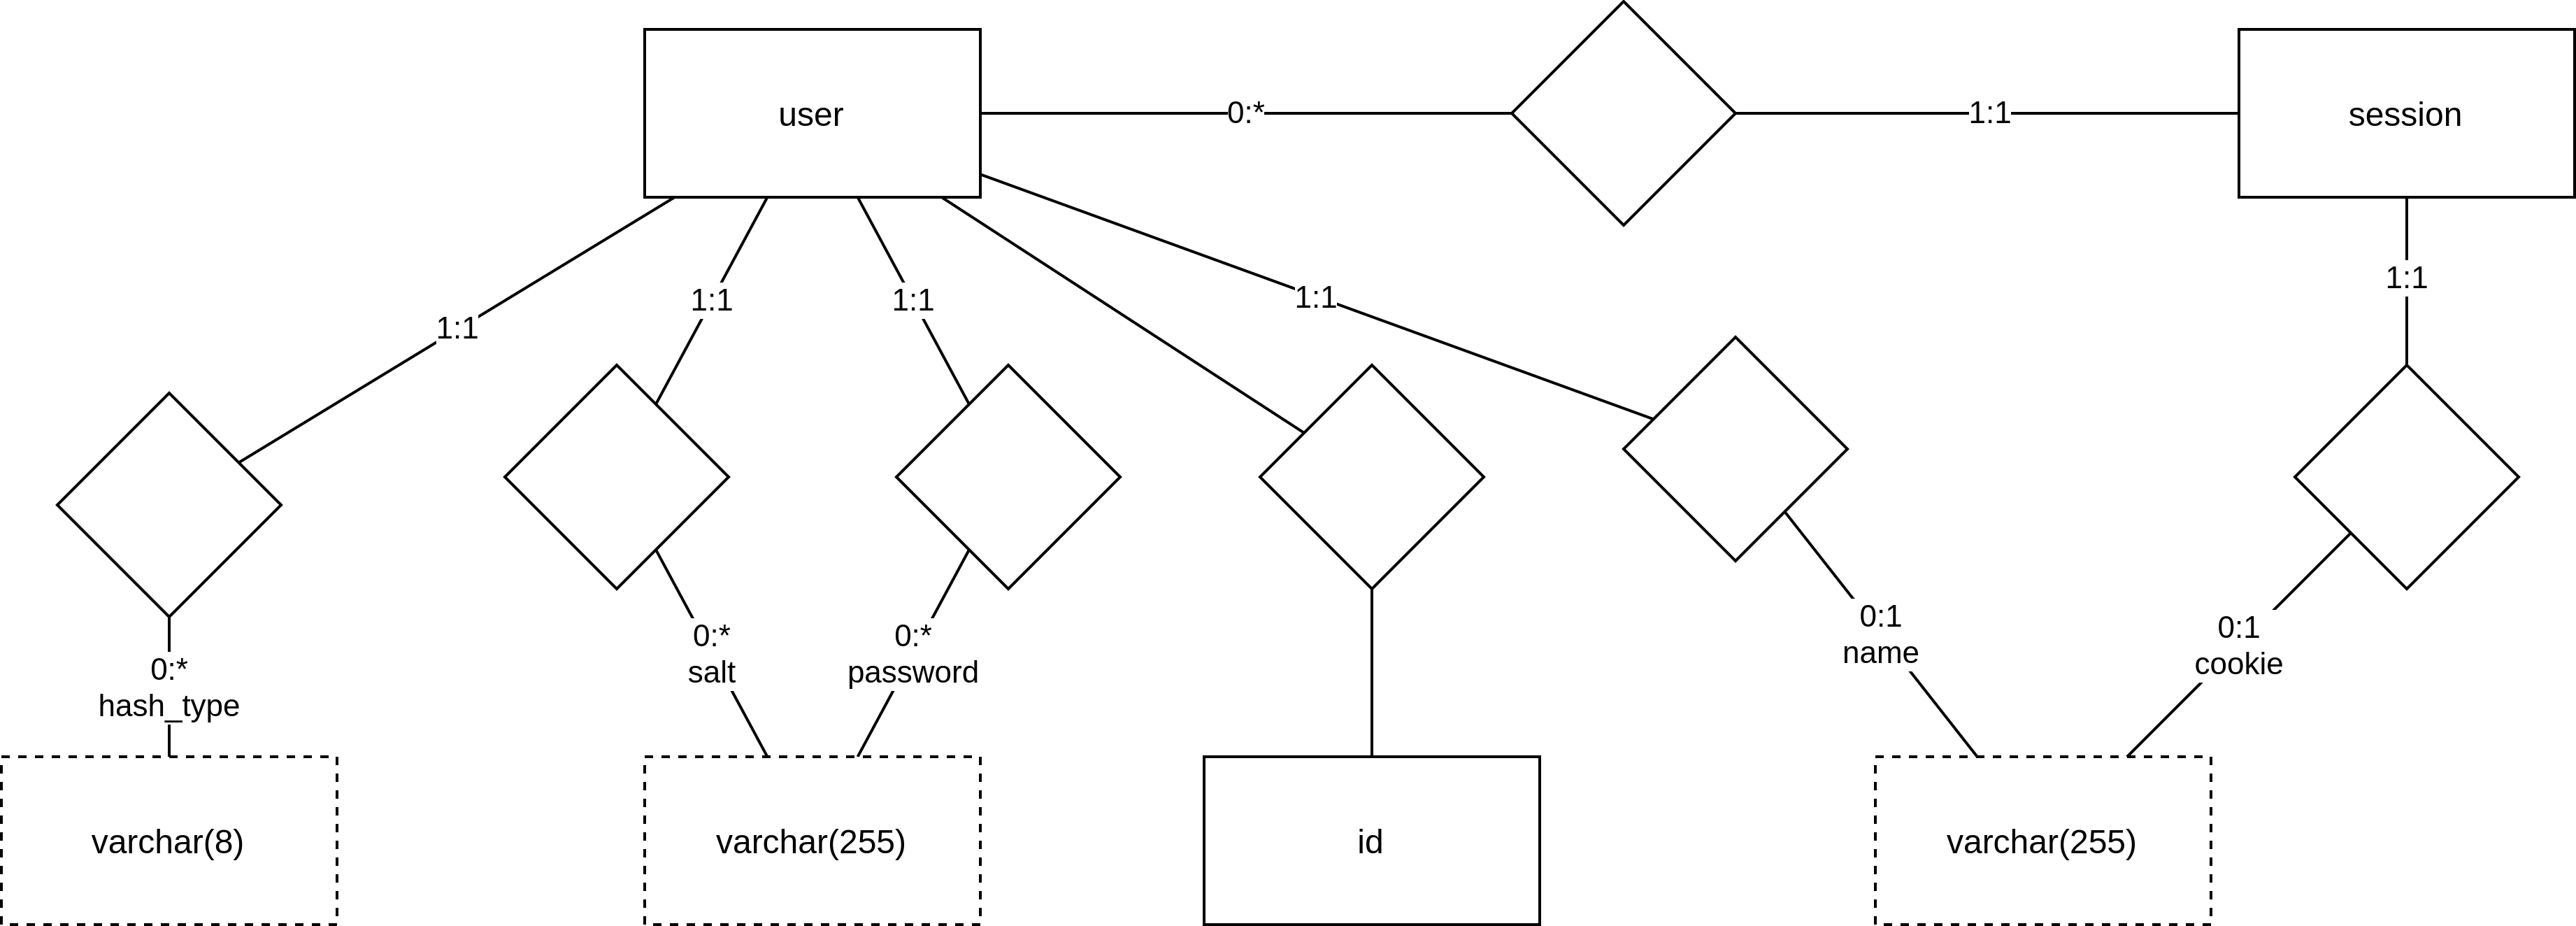
\includegraphics[width=\textwidth]{images/user-db.png}
	\caption{Benutzertabelle mit Cookie-Session}
	\label{fig:user-db}
\end{figure}

\begin{sidewaysfigure}
	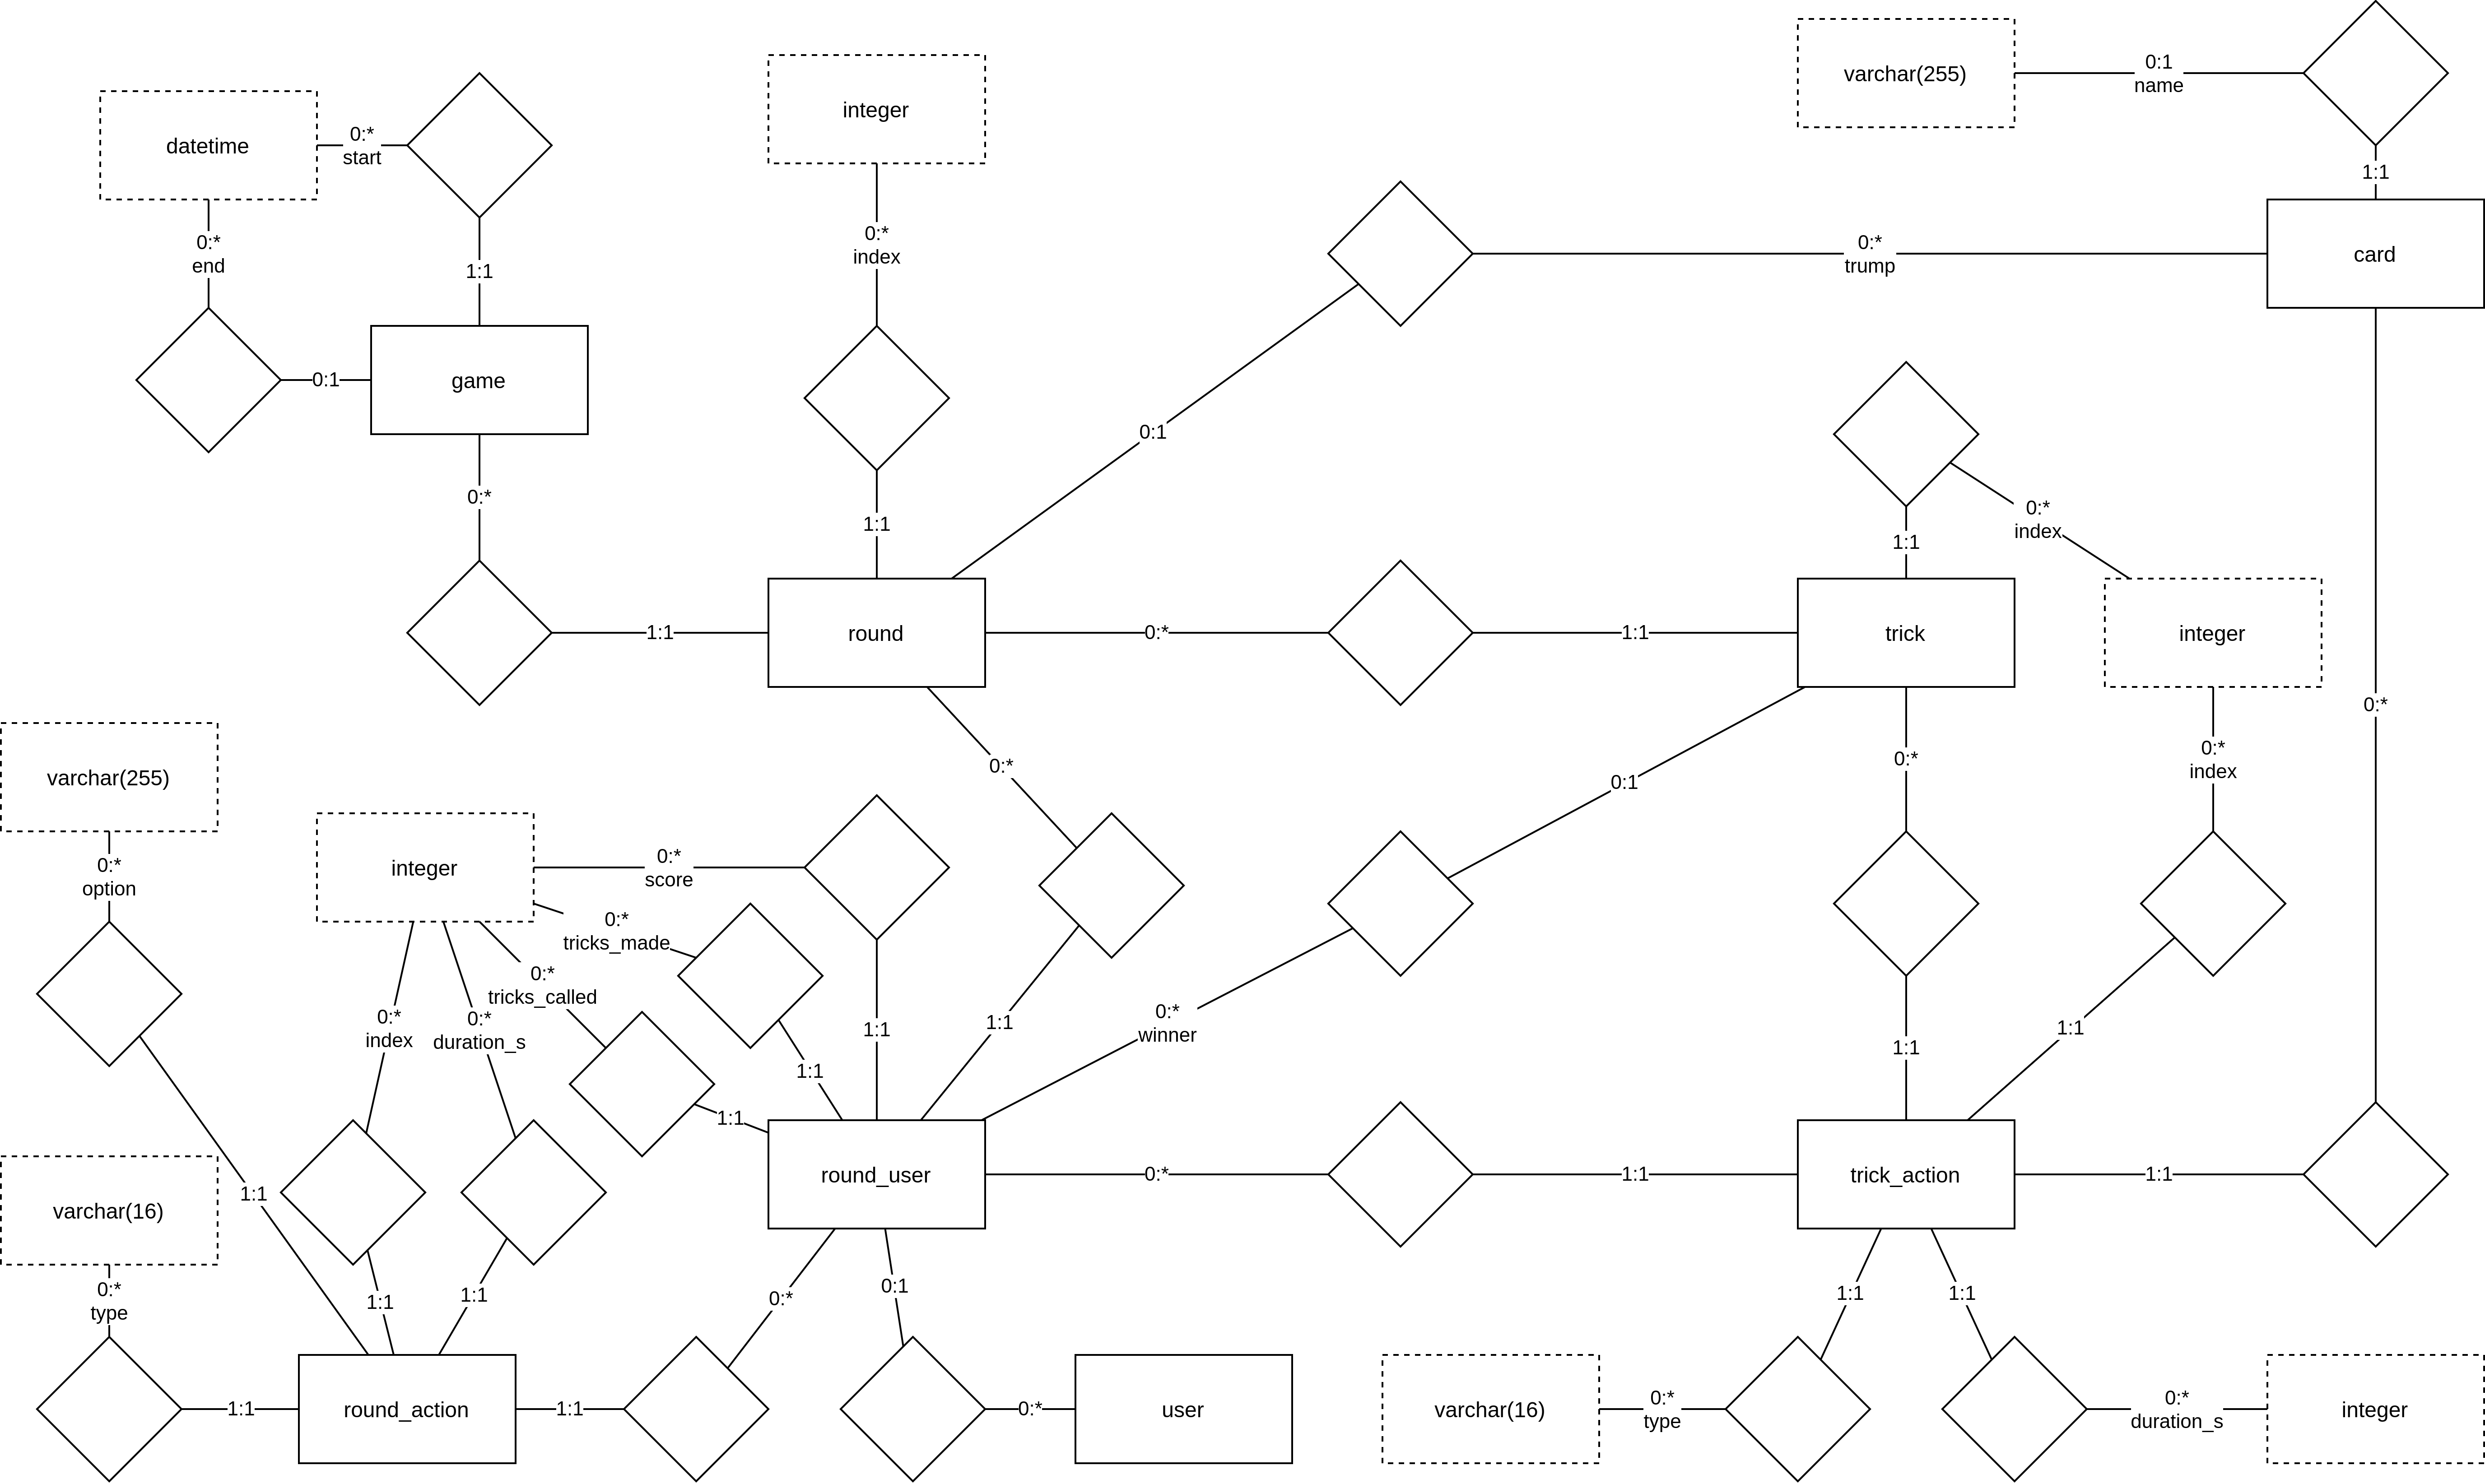
\includegraphics[width=\textheight]{images/statistics-db.png}
	\caption{Datenbankmodel der Statistiken}
	\label{fig:statistics-db}
\end{sidewaysfigure}

\section{Frontend}
Wenn die Frontend-Webseite zum ersten Mal aufgerufen wird, wird das Login-Interface angezeigt. Hierbei muss der Nutzer Name und Passwort eingeben. Optional kann festgelegt werden, ob der Nutzer angemeldet bleiben möchte um eine erneute Eingabe der Daten zu verhindern. Ohne Anmeldung ist sonst nur die Registrierseite erreichbar, da alles weitere eine erfolgreiche Authentifizierung benötigt.

Nachdem der Spieler authentifiziert wurde, wird dieser auf die Lobby-Seite weitergeleitet, wo er wahlweise eine neue Lobby erstellen kann oder einer bereits existierenden mittels eines Codes oder Einladungslinks beitreten kann. Der Ersteller der Lobby hat zusätzlich die Möglichkeit vor dem Spielstart den Spielmodus und die gewünschte Rundenanzahl zu ändern. Zur Verfügung stehen die Standardedition, sowie die beiden Jubiläumseditionen für jeweils 20 und 25 Jahre. Die Rundenanzahl reicht von mindestens einer bis hin zu Anzahl der Karten durch die Anzahl der Spieler. Des Weiteren hat der Lobby-Master die Möglichkeit das Spiel zu starten oder die Lobby über das rechte obere Menü aufzulösen (siehe \cref{fig:lobby}).

\begin{figure}[h]
	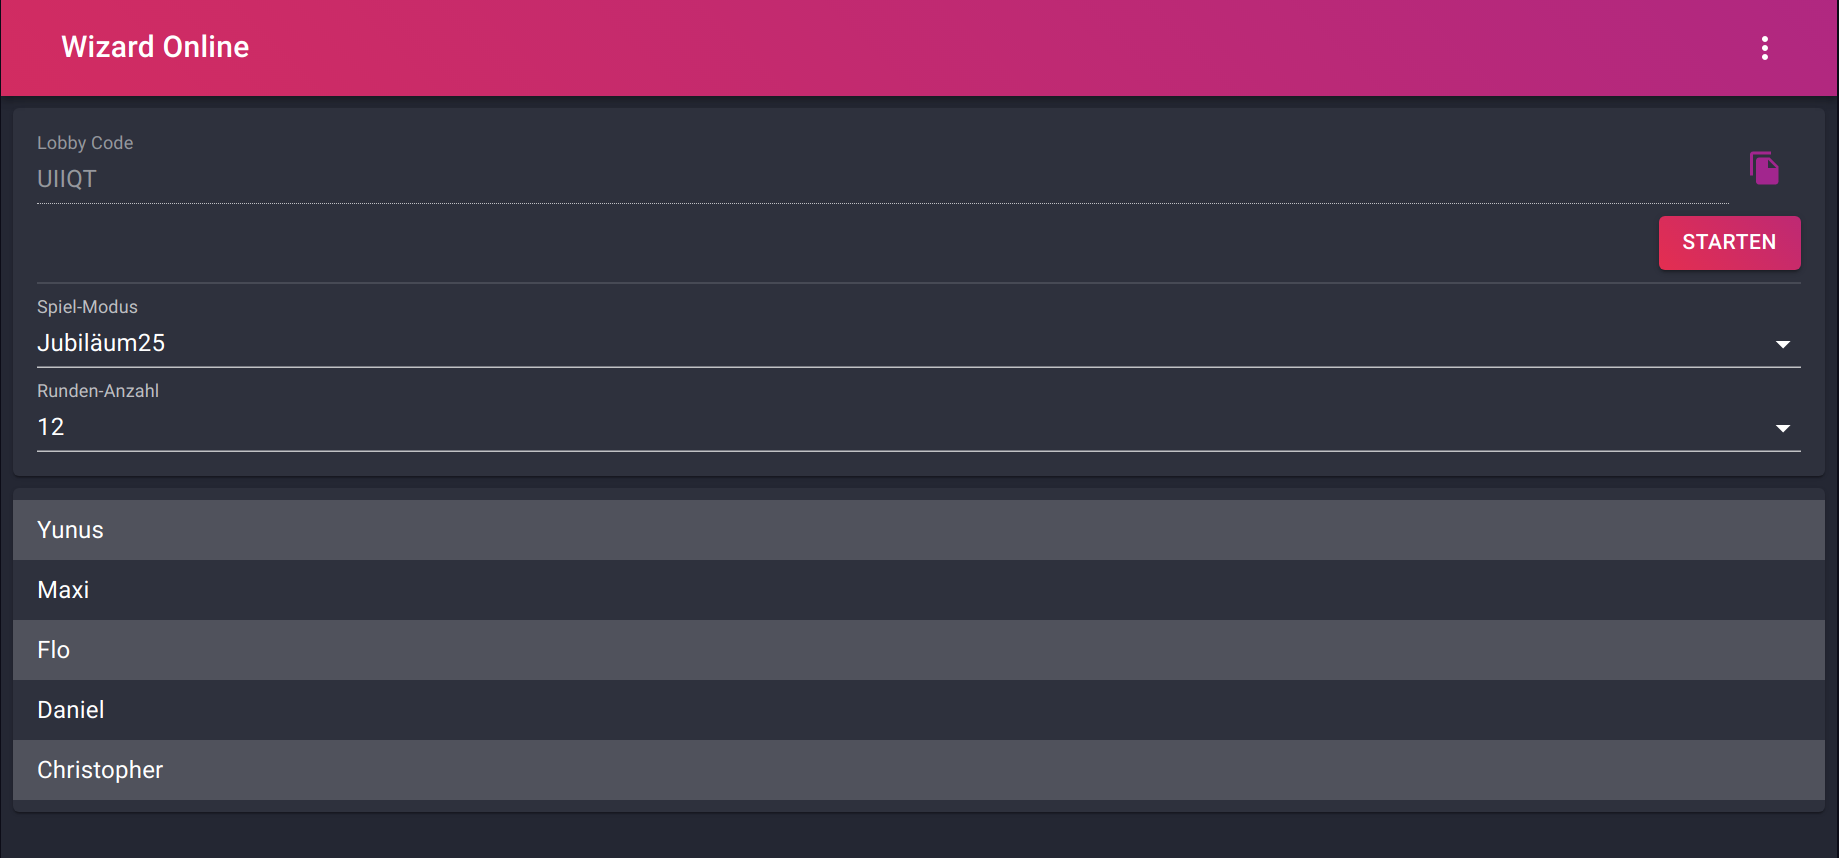
\includegraphics[width=\textwidth]{images/lobby.png}
	\caption{Lobby aus Ersteller Sicht mit mehreren Spielern}
	\label{fig:lobby}
\end{figure}

\begin{wrapfigure}{l}{5cm}
	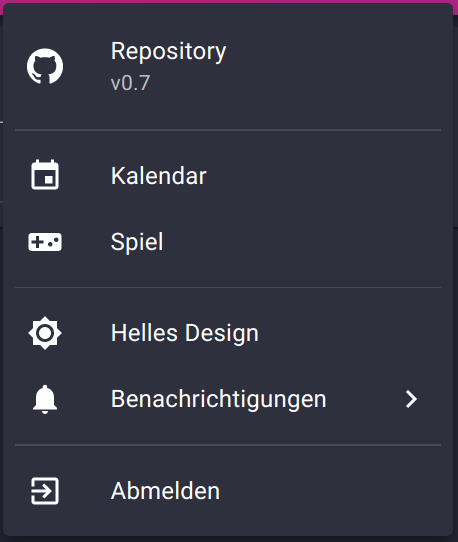
\includegraphics[width=5cm]{images/menu.png}
	\caption{Allgemein verfügbares Menü}
	\label{fig:menu}
\end{wrapfigure}

Das Menü bietet den Nutzern über die ganze Seite verschiedene Schnellaktionen, wie beispielsweise das Springen zwischen den unterschiedlichen Seiten oder auch gewisse Einstellungsmöglichkeit, wie Darstellung und Benachrichtigungen (siehe \cref{fig:menu}). Zusätzlich kann ein angemeldeter Nutzer auch hierdurch sich abmelden oder eine eventuelle Lobby beziehungsweise laufendes Spiel verlassen.

Während dem Spiel werden den Spieler in der Mitte die gespielten Karten angezeigt (siehe \cref{fig:game-view}), welche durch ein Mausklick ausführlicher hervorgehoben werden. Links davon befinden sich zwei halbierte Karten, wobei die obere die Trumpfkarte und die untere die angespielte Karte beschreibt. Die farblichen Umrandungen zeigen jeweils die Trumpf- und angespielte Farbe an. Auf der rechten Seite befindet sich eine Tabelle mit allen Spielern in richtiger Reihenfolge. Hierbei wird links vom Namen der aktuelle Punktestand und rechts die Anzahl der Stiche angezeigt. Zusätzlich wird der für den derzeitigen Stich gewinnende Spieler unterstrichen. Des Weiteren werden alle Spieler, welche eine Aktion, wie beispielsweise die Ansage der Stiche (siehe \cref{fig:trick-selection}) oder anderweitige spezielle Auswahlmöglichkeiten (siehe \cref{fig:trick-color-selection}, \cref{fig:cloud-effect} und \cref{fig:cloud-select}) zur Verfügung haben, farblich hervorgehoben. Die untere Hälfte zeigt die Hand des Spielers an, wobei hier Karten ausgegraut werden, falls diese nicht gespielt werden dürfen (siehe \cref{fig:greyed-out}). Ab der zweiten Runde taucht in der oberen linken Ecke ein Verlauf-Icon auf, welches durch den Fokus des Mauszeigers die gespielten Karten der letzten Stichrunde anzeigen (siehe \cref{fig:last-round}).

\begin{figure}[h]
	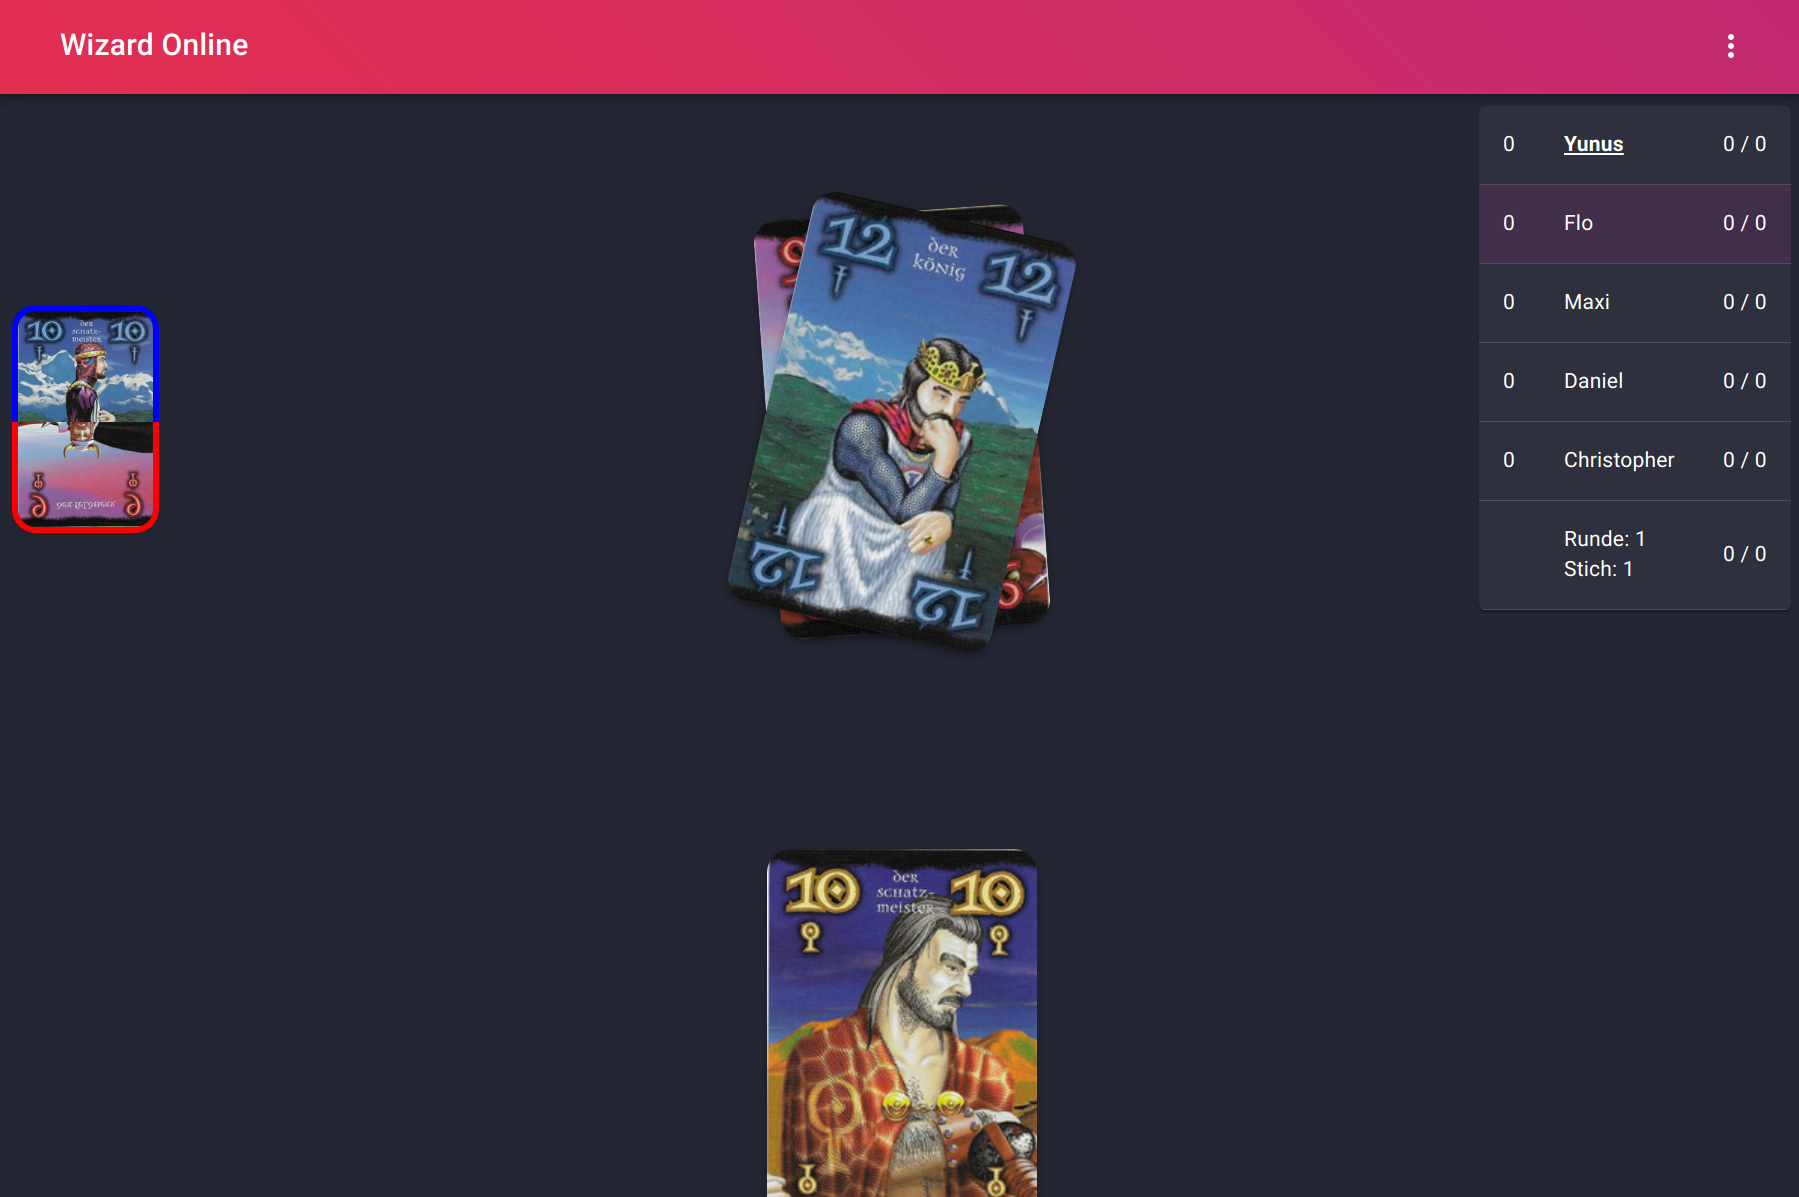
\includegraphics[width=\textwidth]{images/game.png}
	\caption{Spielansicht}
	\label{fig:game-view}
\end{figure}

\begin{figure}[h]
	\begin{minipage}{0.5\textwidth}
		\centering
		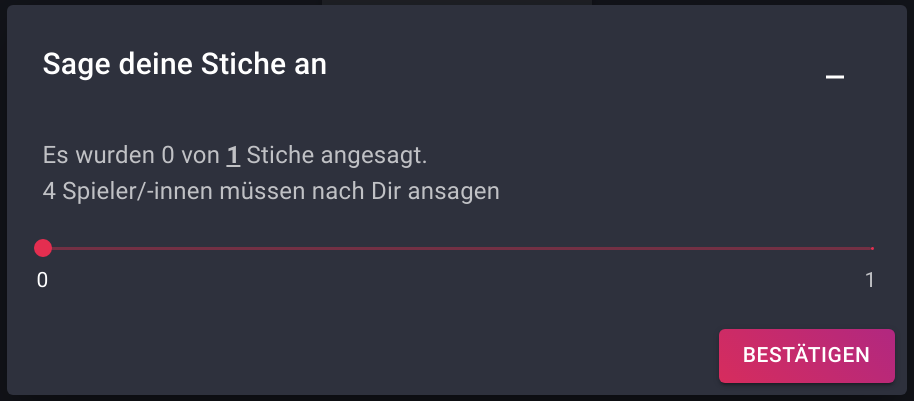
\includegraphics[width=0.95\textwidth]{images/trick-selection.png}
		\caption{Ansage der Stiche}
		\label{fig:trick-selection}
	\end{minipage}
	\begin{minipage}{0.5\textwidth}
		\centering
		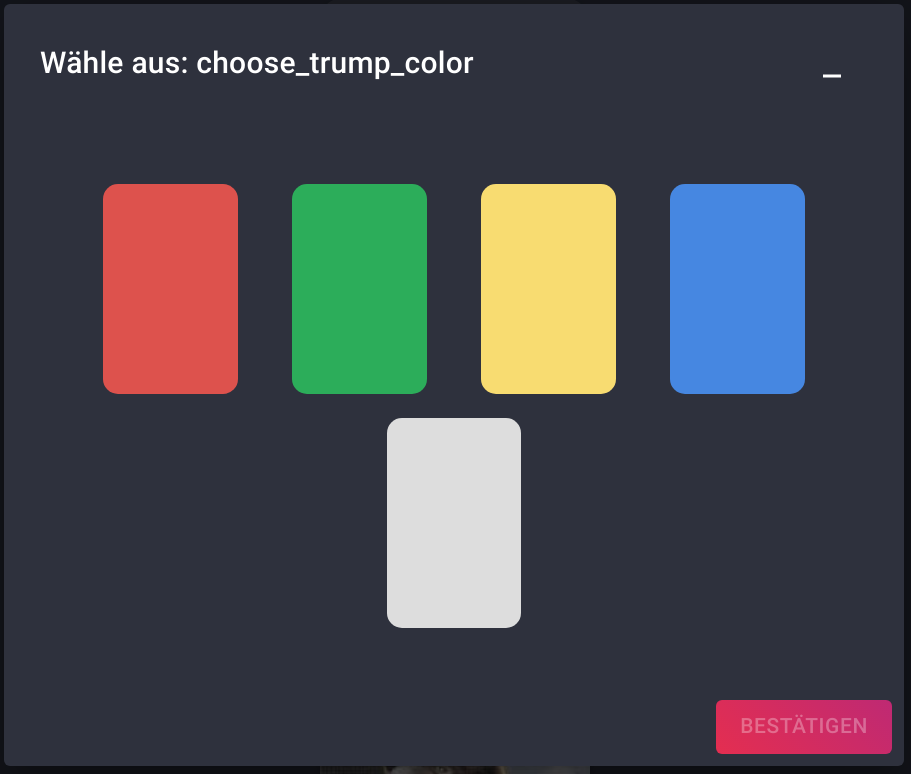
\includegraphics[width=0.95\textwidth]{images/trick-color-selection.png}
		\caption{Auswahl der gewünschten Trumpffarbe}
		\label{fig:trick-color-selection}
	\end{minipage}
\end{figure}

\begin{figure}[h]
	\begin{minipage}{0.5\textwidth}
		\centering
		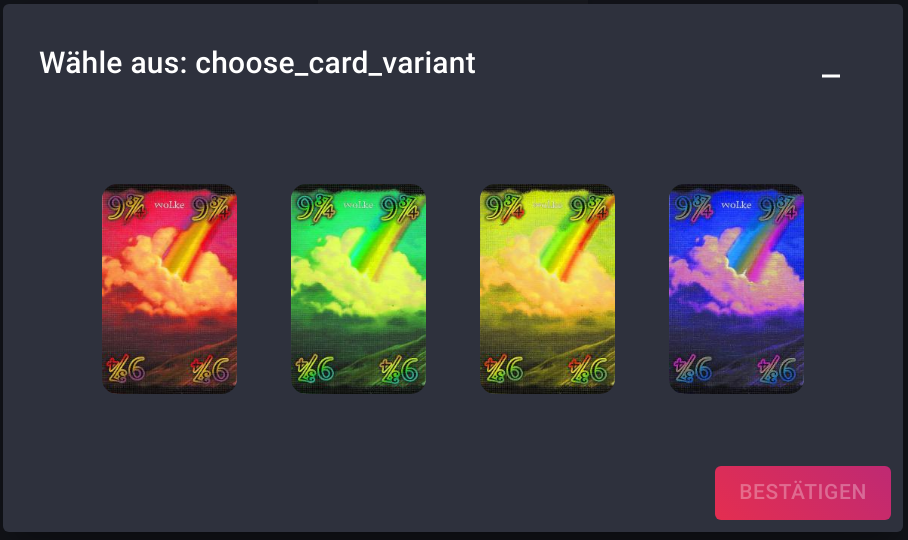
\includegraphics[width=0.95\textwidth]{images/cloud-select.png}
		\caption{Auswahl für die Spezialkarte \textit{Die Wolke}}
		\label{fig:cloud-select}
	\end{minipage}
	\begin{minipage}{0.5\textwidth}
		\centering
		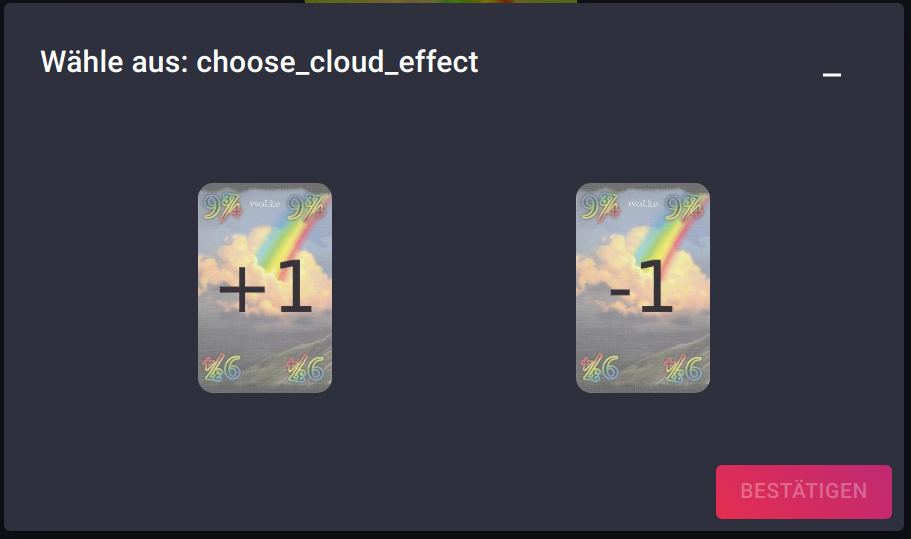
\includegraphics[width=0.95\textwidth]{images/cloud-effect.png}
		\caption{Auswahl für die Auswirkung der Karte \textit{Die Wolke}}
		\label{fig:cloud-effect}
	\end{minipage}
\end{figure}

\begin{figure}[h]
	\centering
	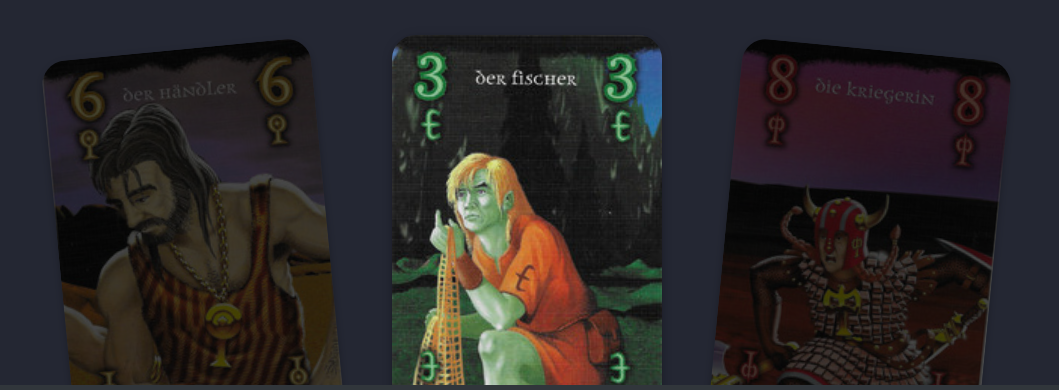
\includegraphics[height=5cm]{images/greyed-out.png}
	\caption{Spielerhand mit ausgegrauten und nicht spielbaren Karten}
	\label{fig:greyed-out}
\end{figure}

\begin{figure}[h]
	\centering
	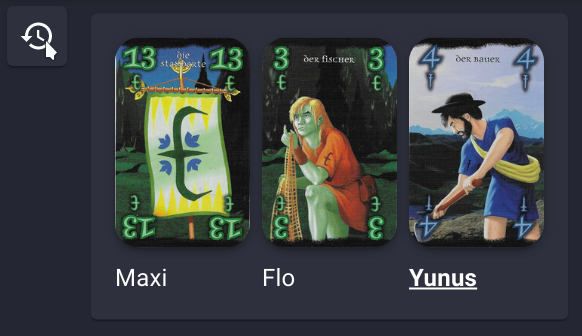
\includegraphics[height=5cm]{images/last-round.png}
	\caption{Gespielte Karten der letzten Stichrunde}
	\label{fig:last-round}
\end{figure}

Zusätzlich kann ein angemeldeter Nutzer über das Menü auf den Kalender zugreifen. Hierbei kann über einfaches Klicken und Ziehen der Maus ein Event erstellt werden, was für alle anderen Spieler sichtbar ist. Diese können je nach Wunsch mit einem Klick beitreten oder es auch verlassen. Sobald keine Spieler in einem Event sind, wird dieses gelöscht. Des Weiteren werden alle Events, welche älter als eine Stunde sind automatisch aus der Datenbank entfernt. Der Sinn des Kalenders ist es Spieler schnell über das Portal zu vernetzten und somit eine einfachere Terminfindung zu ermöglichen.

\label{sec:frontend-registrierung}
Bevor das Passwort in einen Anmeldeschlüssel umgewandelt wird, wird zuerst mithilfe des kostenlosen Dienstes \textit{Have I Been Pwned?} überprüft ob das Passwort in der Vergangenheit kompromittiert wurde. Hierbei werden nur die ersten fünf Zeichen des Passwort-Hashes an den Service geschickt, wodurch das eigentliche Passwort niemals den Browserkontext verlässt. Falls die Abfrage erfolgreich verlief wird dem Benutzer eine Benachrichtigung mit der Anzahl der Kompromittierungen angezeigt und das Passwort abgewiesen. Anschließend wird ein 64-Bit langer Salt zufällig generiert, welcher mithilfe der \gls{pbkdf2} + SHA512 Methode und dem eigentlichen Passwort einen 256-Bit langen Schlüssel generiert. Für den Abschluss wird die entsprechende API Funktion \textit{register} mit den Base64 enkodierten Schlüssel und Salt aufgerufen.
